% vim: spell:spelllang=en:
\documentclass[12pt, oneside]{article}
\usepackage[a4paper, left=2.5cm, right=2.5cm, top=2.5cm, bottom=2.5cm]{geometry}

\usepackage[utf8]{inputenc} % Use unicode
\usepackage[T1]{fontenc}
\usepackage[catalan]{babel} % Names in spanish

%% Bibliography:
%\usepackage{comment}
%\usepackage[
    %backend=biber,
    %style=numeric,
%]{biblatex}
%\DeclareNameAlias{default}{last-first}

%\usepackage{csquotes}       % For bibliography quotations
%\DeclareQuoteAlias{spanish}{catalan}

%\addbibresource{biblio.bib}
%% see:
%% https://www.sharelatex.com/learn/Bibliography_management_in_LaTeX#The_bibliography_file

%\usepackage{datetime} % Customize date
%% \monthyeardate\today gives the date without the day
%\newdateformat{monthyeardate}{%
    %\monthname[\THEMONTH], \THEYEAR}

% For cross references
\usepackage[colorlinks = true]{hyperref}
\usepackage[catalan]{varioref}
%\usepackage{cleveref}
%hyperref configuration so that it doesn't contrast so much colorlinks,
\hypersetup{
   linkcolor={black},
   citecolor={black},
   %linkcolor={red!50!black},
   %citecolor={blue!50!black},
   urlcolor={blue!80!black}
}

\usepackage{mathtools}  % amsmath + more
\usepackage{amsthm}     % Theorem enviroment
\usepackage{amssymb}    % More symbols
\usepackage{amstext}    % Text inside mathenv

\usepackage{relsize}    % Bigger math with mathlarger{___}
\usepackage{nicefrac}   % nice fractions in one line

\usepackage[export]{adjustbox}  % Adjust table size
\usepackage{float}              % Force tables and images position (H and H!)
\usepackage{wrapfig}            % Wrap images like in HTML

\usepackage{tabularx, colortbl, booktabs}    % Better tables
\usepackage{longtable}                      % Multiple page table

% Split cell in lines and more formating options inside table
\usepackage{array, multirow, multicol, makecell}

%\usepackage{subcaption}                     % Subfigures
%\usepackage[framemethod=tikz]{mdframed}     % Custom frames

%\usepackage[bottom]{footmisc} % Footnotes at bottom of page

%\usepackage[alsoload=hep]{siunitx}          % SI units and uncertainties
%\sisetup{locale = FR}                       % Commas and so on for spanish
%\sisetup{separate-uncertainty=true}
%\sisetup{
  %per-mode=fraction,
  %fraction-function=\nicefrac
%}

%\usepackage{tikz}
%%\usetikzlibrary{arrows}
%%\usetikzlibrary{scopes}
%\usetikzlibrary{babel}

%\usepackage{listings}       % For code blocks

%% Custom code highlight
%\definecolor{codegreen}{rgb}{0,0.6,0}
%\definecolor{codegray}{rgb}{0.5,0.5,0.5}
%\definecolor{codepurple}{rgb}{0.58,0,0.82}
%\definecolor{backcolour}{rgb}{0.95,0.95,0.92}
%\definecolor{lightblue}{RGB}{135,206,250}

%\lstdefinestyle{mystyle}{ backgroundcolor=\color{backcolour},
    %commentstyle=\color{codegreen}, keywordstyle=\color{blue},
    %numberstyle=\tiny\color{codegray}, stringstyle=\color{red},
    %identifierstyle=\color{black}, basicstyle=\footnotesize,
    %%breakatwhitespace=false,
    %breaklines=true,
    %%captionpos=b,                    keepspaces=true,
    %numbers=left,                    numbersep=5pt,
    %showspaces=false,
    %%showstringspaces=false, showtabs=false,
    %tabsize=4
%}
%\lstset{style=mystyle}

\newcommand{\whitepage}{
    \clearpage\thispagestyle{empty}\addtocounter{page}{-1} \newpage \clearpage
}

% Add command before appendix session for page numbering: A-1
%\newcommand{\appendixpagenumbering}{
    %\break
    %\pagenumbering{arabic}
    %\renewcommand{\thepage}{\thesection-\arabic{page}}
%}

%% Custom Math operators (functions not in italic in math mode):
%\DeclareMathOperator{\arcsec}{arcsec}
%\DeclareMathOperator{\arccot}{arccot}
%\DeclareMathOperator{\arccsc}{arccsc}
%\DeclareMathOperator{\cis}{cis}


\usepackage{caption}
\usepackage{subcaption}
\usepackage{graphicx}

\usepackage{siunitx}

\renewcommand\theadfont{\bfseries}

\title{
    PAR Laboratory Assignment\\
    Lab 1: Experimental setup and tools
}

\author{
    par2109:
    Aleix Boné,
    Alex Herrero
}

\date{
    Spring 2019-20
}

\begin{document}

\thispagestyle{empty}
\clearpage
\setcounter{page}{-1}

\begin{titlepage}
{
    \centering
    \null
    \vfill
    {\Huge \bfseries PAR Laboratory Assignment\par}
    \vspace{3em}
    {\Large {\scshape Lab 1:} Experimental setup and tools\par}
    \vfill
\begin{center}
\end{center}
    \vspace{3cm}

    \vfill
    {\raggedleft \Large
        Aleix Boné\\
        Alex Herrero\\
        {\bfseries\ttfamily par2109}\\
        \vspace{4em}
        2020-03-06
        \par}
}
\end{titlepage}

\pagebreak

%After the last session for this laboratory assignment, and before starting the
%next one, you will have to deliver a report in PDF format (other formats will
%not be accepted) describing the results and conclusions that you have obtained
%when doing the assignment. As part of the document, you will have to include
%any code fragment, figure or plot you need to support your explanations. Your
%professor will open the assignment at the Raco website and set the appropriate
%delivery dates for the delivery. Only one file has to be submitted per group
%through the Raco website.
%
%Important: In the front cover of the document, please clearly state the name of
%all components of the group, the identifier of the group (username parXXYY),
%title of the assignment, date, academic


\pagebreak
\tableofcontents
\pagebreak
\pagenumbering{arabic} 

\section{Node architecture and memory}%
\label{sec:node_architecture_and_memory}

%Describe the architecture of the boada server. To accompany your description,
%you should refer to the following table summarising the relevant architectural
%characteristics of the different node types available:

The boada server consists of 8 different nodes with different processors. As we can see in
the table~\ref{tab:node_arch_and_mem} there are 3 different architectures with slight variations
\texttt{boada-1 to boada-4} have the same number of sockets(2), cores(6) and threads per core (2), which adds up to a total of 24 threads.

\texttt{boada-5} has the same number of sockets, threads and cores as the previous \texttt{boadas} but with higher Maximum core frequency and a much larger shared cache size and Main memory.
The output of \texttt{lstopo} also shows us that it has 4 \texttt{GPUs}.

\texttt{boada-6 to boada-8} have 8 cores per socket but only one thread per core (amounting to 16 threads instead of the 24 of the other nodes) and a much lower clock frequency. However it has the
highest last-level cache size.

\begin{table}[H]%
    \centering
    \begin{tabular}{lrrr}

    \toprule
        & \texttt{boada 1 to 4} & \texttt{boada 5} & \texttt{boada 6 to 8} \\
    \midrule
        Number of sockets per node          & 2        & 2        & 2        \\
        Number of cores per socket          & 6        & 6        & 8        \\
        Number of threads per core          & 2        & 2        & 1        \\
        Maximum core frequency              & 2395 MHz & 2600 MHz & 1700 MHz \\
    \addlinespace[1em]
        L1-I cache size (per-core)          & 32K      & 32K      & 32K      \\
        L1-D cache size (per-core)          & 32K      & 32K      & 32K      \\
        L2 cache size (per-core)            & 256K     & 256K     & 256K     \\
        Last-level cache size (per-socket)  & 12288K   & 15360K   & 20480K   \\
    \addlinespace[1em]
        Main memory size (per socket)       & 12 Gb    & 31 Gb    & 16 Gb    \\
        Main memory size (per node)         & 23 Gb    & 63 Gb    & 31 Gb    \\
    \bottomrule

    \end{tabular}
    
    \caption{Architecture of boada nodes}%
    \label{tab:node_arch_and_mem}
\end{table}

%Also include in the description the architectural diagram for one of the nodes
%boada-1 to boada-4 as obtained when using the lstopo command. Appropriately
%comment whatever you consider appropriate.

In figure~\ref{fig:arch_boada1} we can see the data from table~\ref{tab:node_arch_and_mem} corresponding
to \texttt{boada-1}. The cache L3 is shared between the cores of each socket.
 while the others are local to each core. There is no shared memory between the sockets.

\begin{figure}[H]%
    \centering
    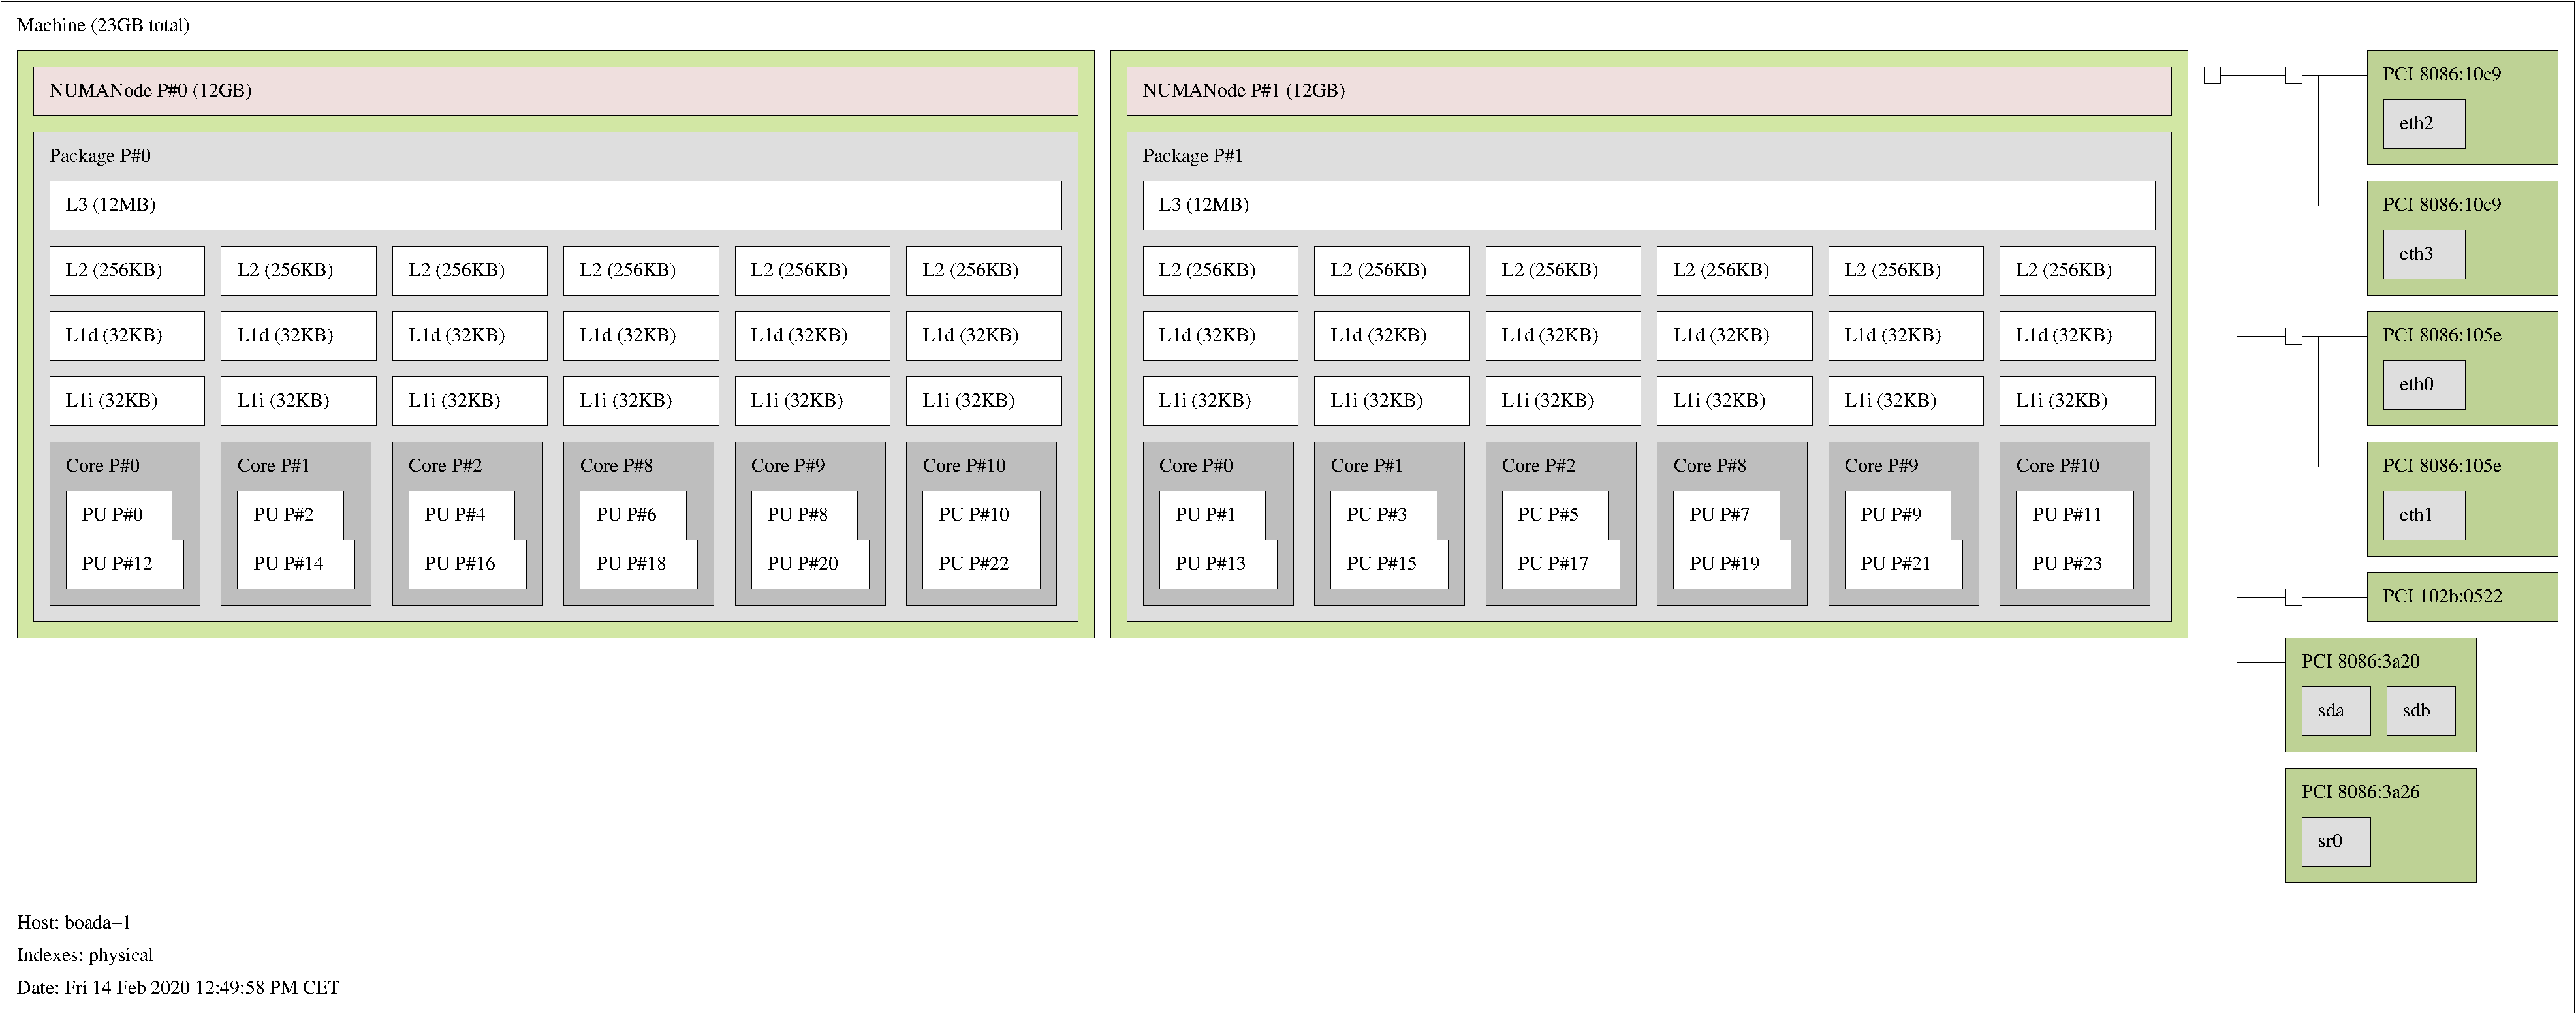
\includegraphics[width=\textwidth]{./data/map-boada-1.pdf}
    \caption{Architectural diagram for \texttt{boada-1}}%
    \label{fig:arch_boada1}
\end{figure}


\section{Strong vs.\ weak scalability}%
\label{sec:strong_vs_weak_scalability}

%Briefly explain what strong and weak scalability refer to. Exemplify your
%explanation using the execution time and speed–up plots that you obtained for
%pi omp.c. Reason about the results obtained.

In strong scalability  the  number  of  threads  is  changed  with  a  fixed  problem  size.   In  this  case parallelism is used to reduce the execution time of the program.

In weak scalability the problem size is proportional to the number of threads. In this case parallelism is used to increase the problem size for which the program is execute

\begin{figure}[H]
\centering
\begin{minipage}{.5\textwidth}
  \centering
  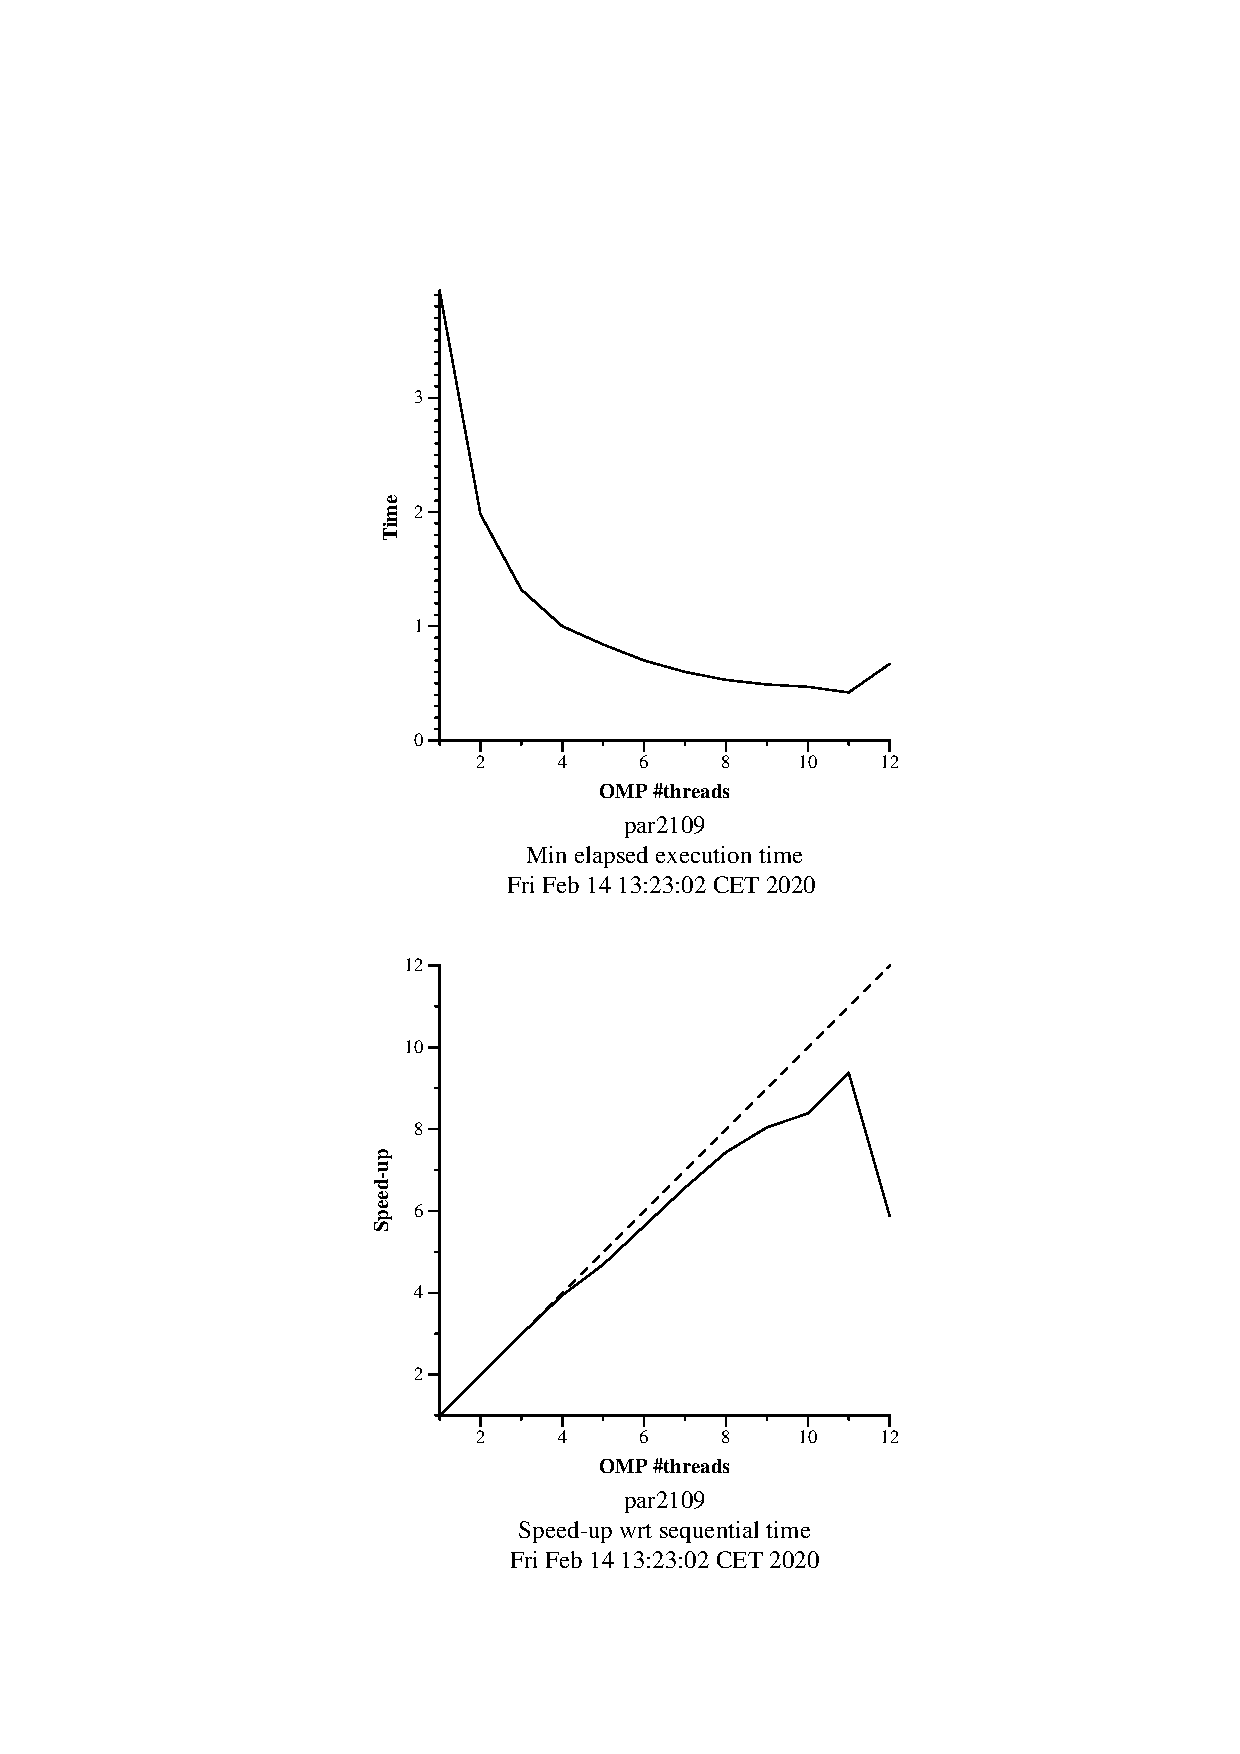
\includegraphics[width=.7\linewidth]{./data/pi/pi_omp-1000000000-1-12-3-strong-boada-2.pdf}
  \captionof{figure}{Strong scalability}
  \label{fig:strong}
\end{minipage}%
\begin{minipage}{.5\textwidth}
  \centering
  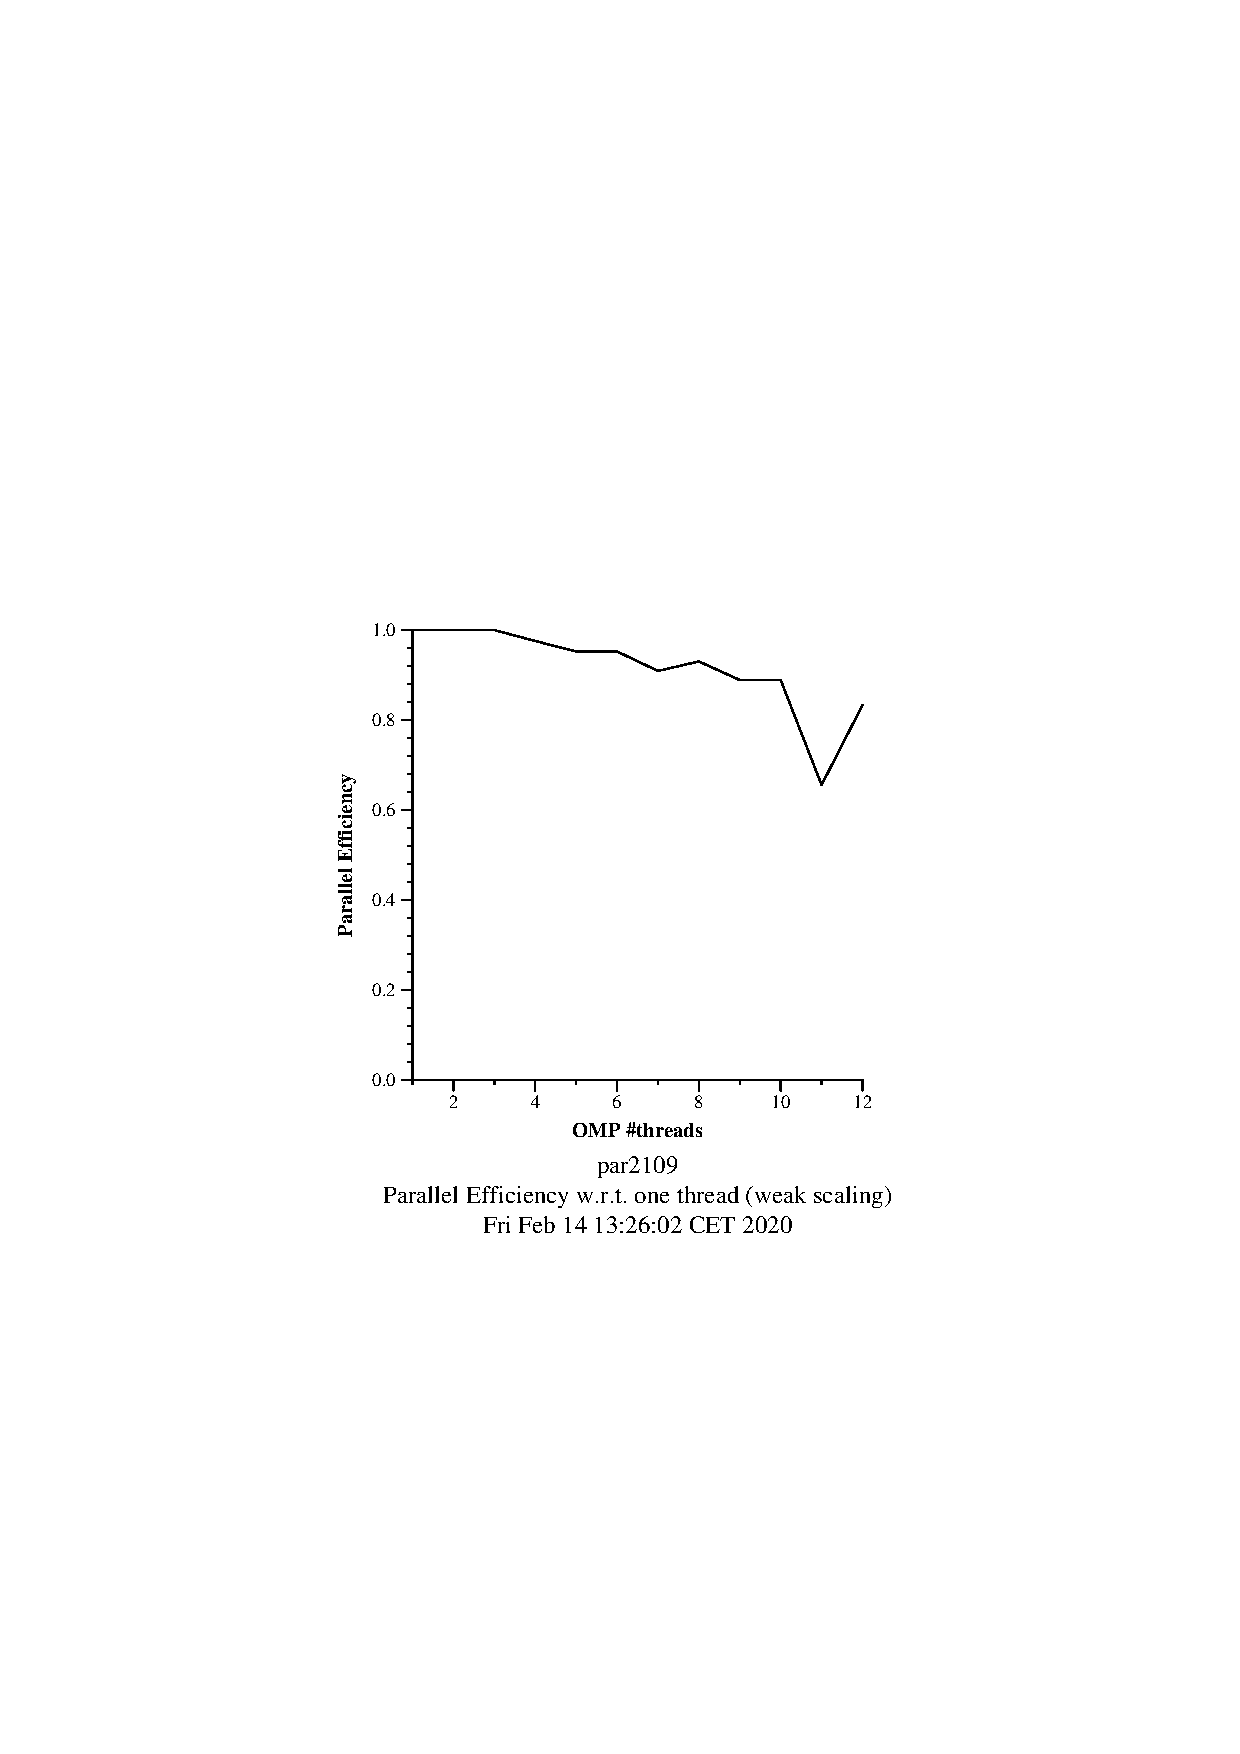
\includegraphics[width=.7\linewidth]{./data/pi/pi_omp-100000000-1-12-3-weak-boada-3.pdf}
  \captionof{figure}{Weak scalability}
  \label{fig:weak}
\end{minipage}
\end{figure}

In strong scalability, as we can observe in figure~\ref{fig:strong}, time decreases as we increase the number of threads and therefore the speedup almost increases linearly. Except in the case we use 12 threads that time and speedup increase because there are threads without doing useful work or the overhead of creating the threads starts to out-weight its benefits


%TODO: finish this
%TODO: razonar sobre los resultados obtenidos

Similarly, in weak scalability (figure~\ref{fig:weak}) we can see that the parallel efficiency remains close to the ideal vale of 1 slowly decreasing and dips at 11 threads. Although the parallel efficiency increases again at 12 threads,
its still significantly lower that the value of 10 threads.


\section{Analysis of task decompositions for \emph{3DFFT}}%
\label{sec:analysis_of_task_decompositions_for_3dfft}

%In this part of the report you should summarise the main conclusions from the
%analysis of task decompositions for the 3DFFT program. Backup your conclusions
%with the following table properly filled in with the information obtained in
%the laboratory session for the initial and different versions generated

\begin{table}[H]%
    \centering
    \begin{tabular}{cS[table-format=9.]S[table-format=9.]S[table-format=2.9]}
    \toprule
    \thead{Version} & {$T_1$} & {$T_\infty$} & {\thead{Parallelism}} \\
    \midrule
    seq     & 639 780 001 &  639 780 001 & 1 \\ % todas las a seran la misma (o deberían)
    v1      & 639 780 001 &  639 707 001 & 1.000 114 115 \\ % c = a/b
    v2      & 639 780 001 &  361 190 001 & 1.771 311 496 \\
    v3      & 639 780 001 &  154 438 001 & 4.142 633 269 \\
    v4      & 639 780 001 &   64 102 001 & 9.980 655 69 \\
    v5      & 639 780 001 &    8 155 001 & 78.452 473 642 \\
    \bottomrule
    \end{tabular}
    \caption{Parallelism for different \texttt{3dfft} versions}
    \label{tab:parallelism}
\end{table}

%TODO: sacar conclusiones

%For versions v4 and v5 of 3dfft tar.c perform an analysis of the potential
%strong scalability that is expected. For that include a plot with the
%execution time and/or speedup when using 1, 2, 4, 8, 16 and 32 processors, as
%reported by the simulation module inside Tareador. You should also include the
%relevant(s) part(s) of the code that help the reader to understand why v5 is
%able to scale to a higher number of processors compared to v4, capturing the
%task dependence graphs that are obtained with Tareador.

Figures~\ref{fig:exec_v4} and \ref{fig:exec_v5} show the change in execution time
with the number of processors. Since its difficult to appreciate the differences with a
linear scale, we have included figures~\ref{fig:exec_v4_log} and \ref{fig:exec_v5_log} with
a logarithmic scale to show how the execution time of \emph{v5} decreases from 16 to 32 processors
and \emph{v4} does not, meaning that \emph{v5} can be further parallelized while we have reached a limit
with \emph{v4}.

\begin{figure}[H]
\centering
\begin{minipage}{.5\textwidth}
  \centering
  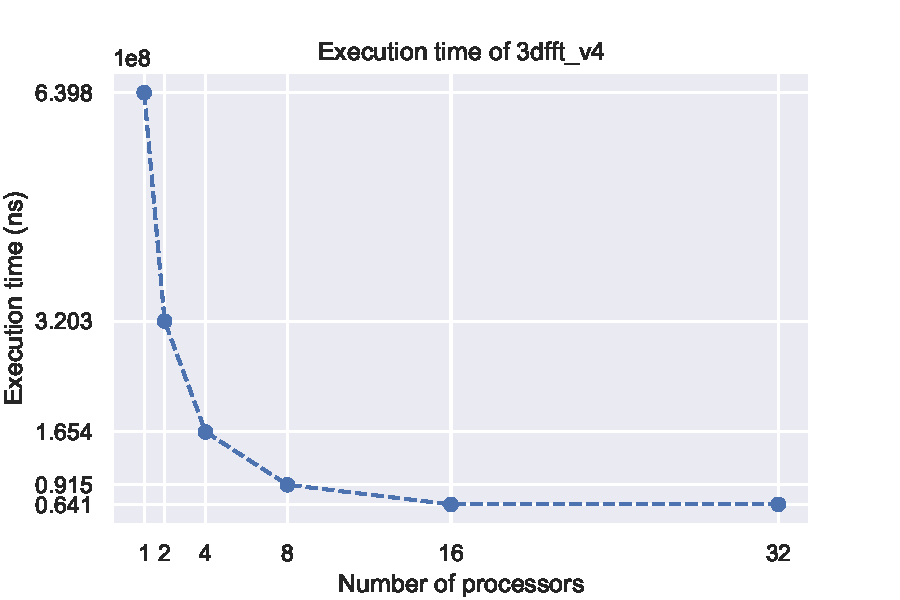
\includegraphics[width=\linewidth]{./data/execution_v4.pdf}
  \captionof{figure}{Execution time of v4}
  \label{fig:exec_v4}
\end{minipage}%
\begin{minipage}{.5\textwidth}
  \centering
  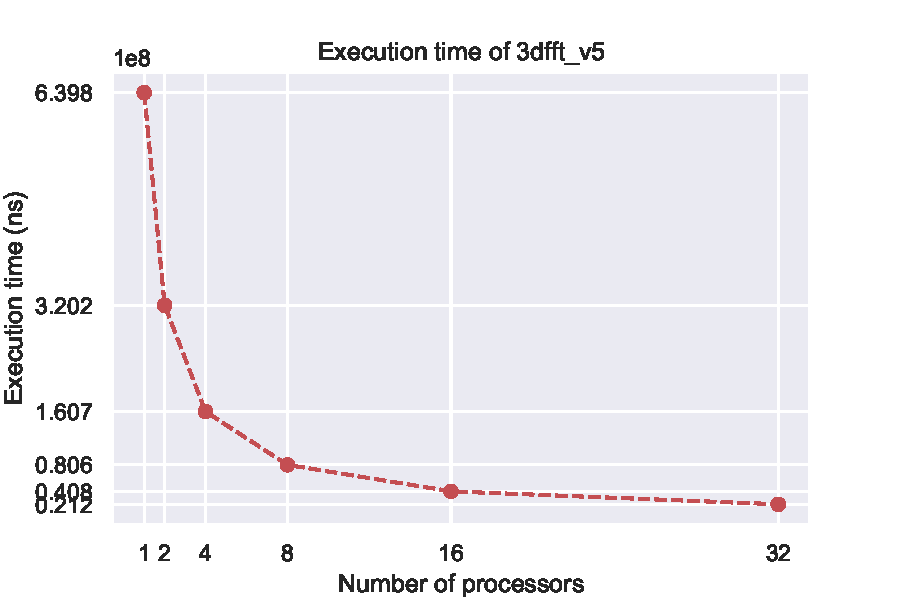
\includegraphics[width=\linewidth]{./data/execution_v5.pdf}
  \captionof{figure}{Execution time of v5}
  \label{fig:exec_v5}
\end{minipage}
\end{figure}


\begin{figure}[H]
\centering
\begin{minipage}{.5\textwidth}
  \centering
  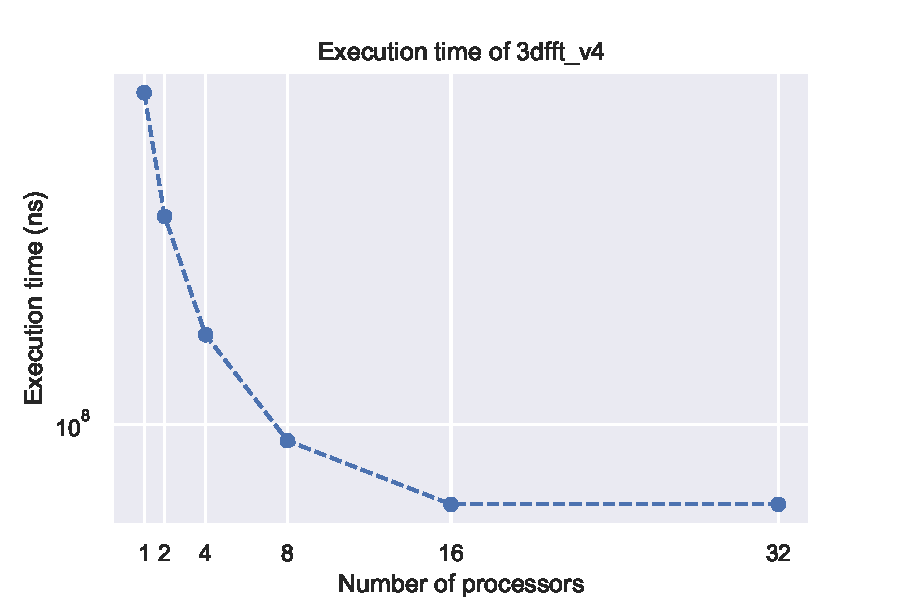
\includegraphics[width=\linewidth]{./data/execution_v4_log.pdf}
  \captionof{figure}{Execution time of v4 (log scale)}
  \label{fig:exec_v4_log}
\end{minipage}%
\begin{minipage}{.5\textwidth}
  \centering
  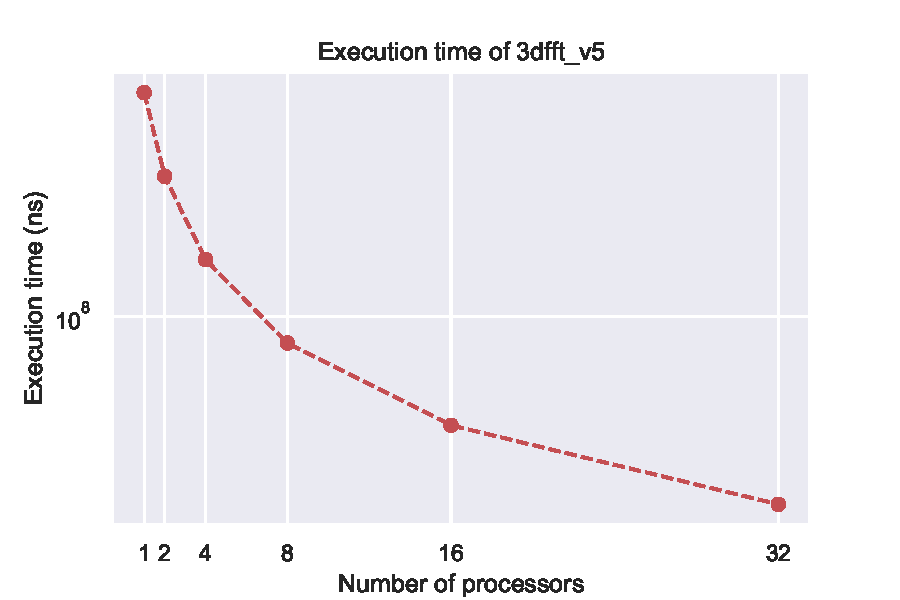
\includegraphics[width=\linewidth]{./data/execution_v5_log.pdf}
  \captionof{figure}{Execution time of v5 (log scale)}
  \label{fig:exec_v5_log}
\end{minipage}
\end{figure}

The task dependency graphs for \emph{v4} (figure~\ref{fig:depen_v4}) and \emph{v5} (figure~\ref{fig:depen_v5}) illustrate that \emph{v5} has much more fine grained tasks that can be parallelized as opposed to \emph{v4}.

\begin{figure}[H]%
    \centering
    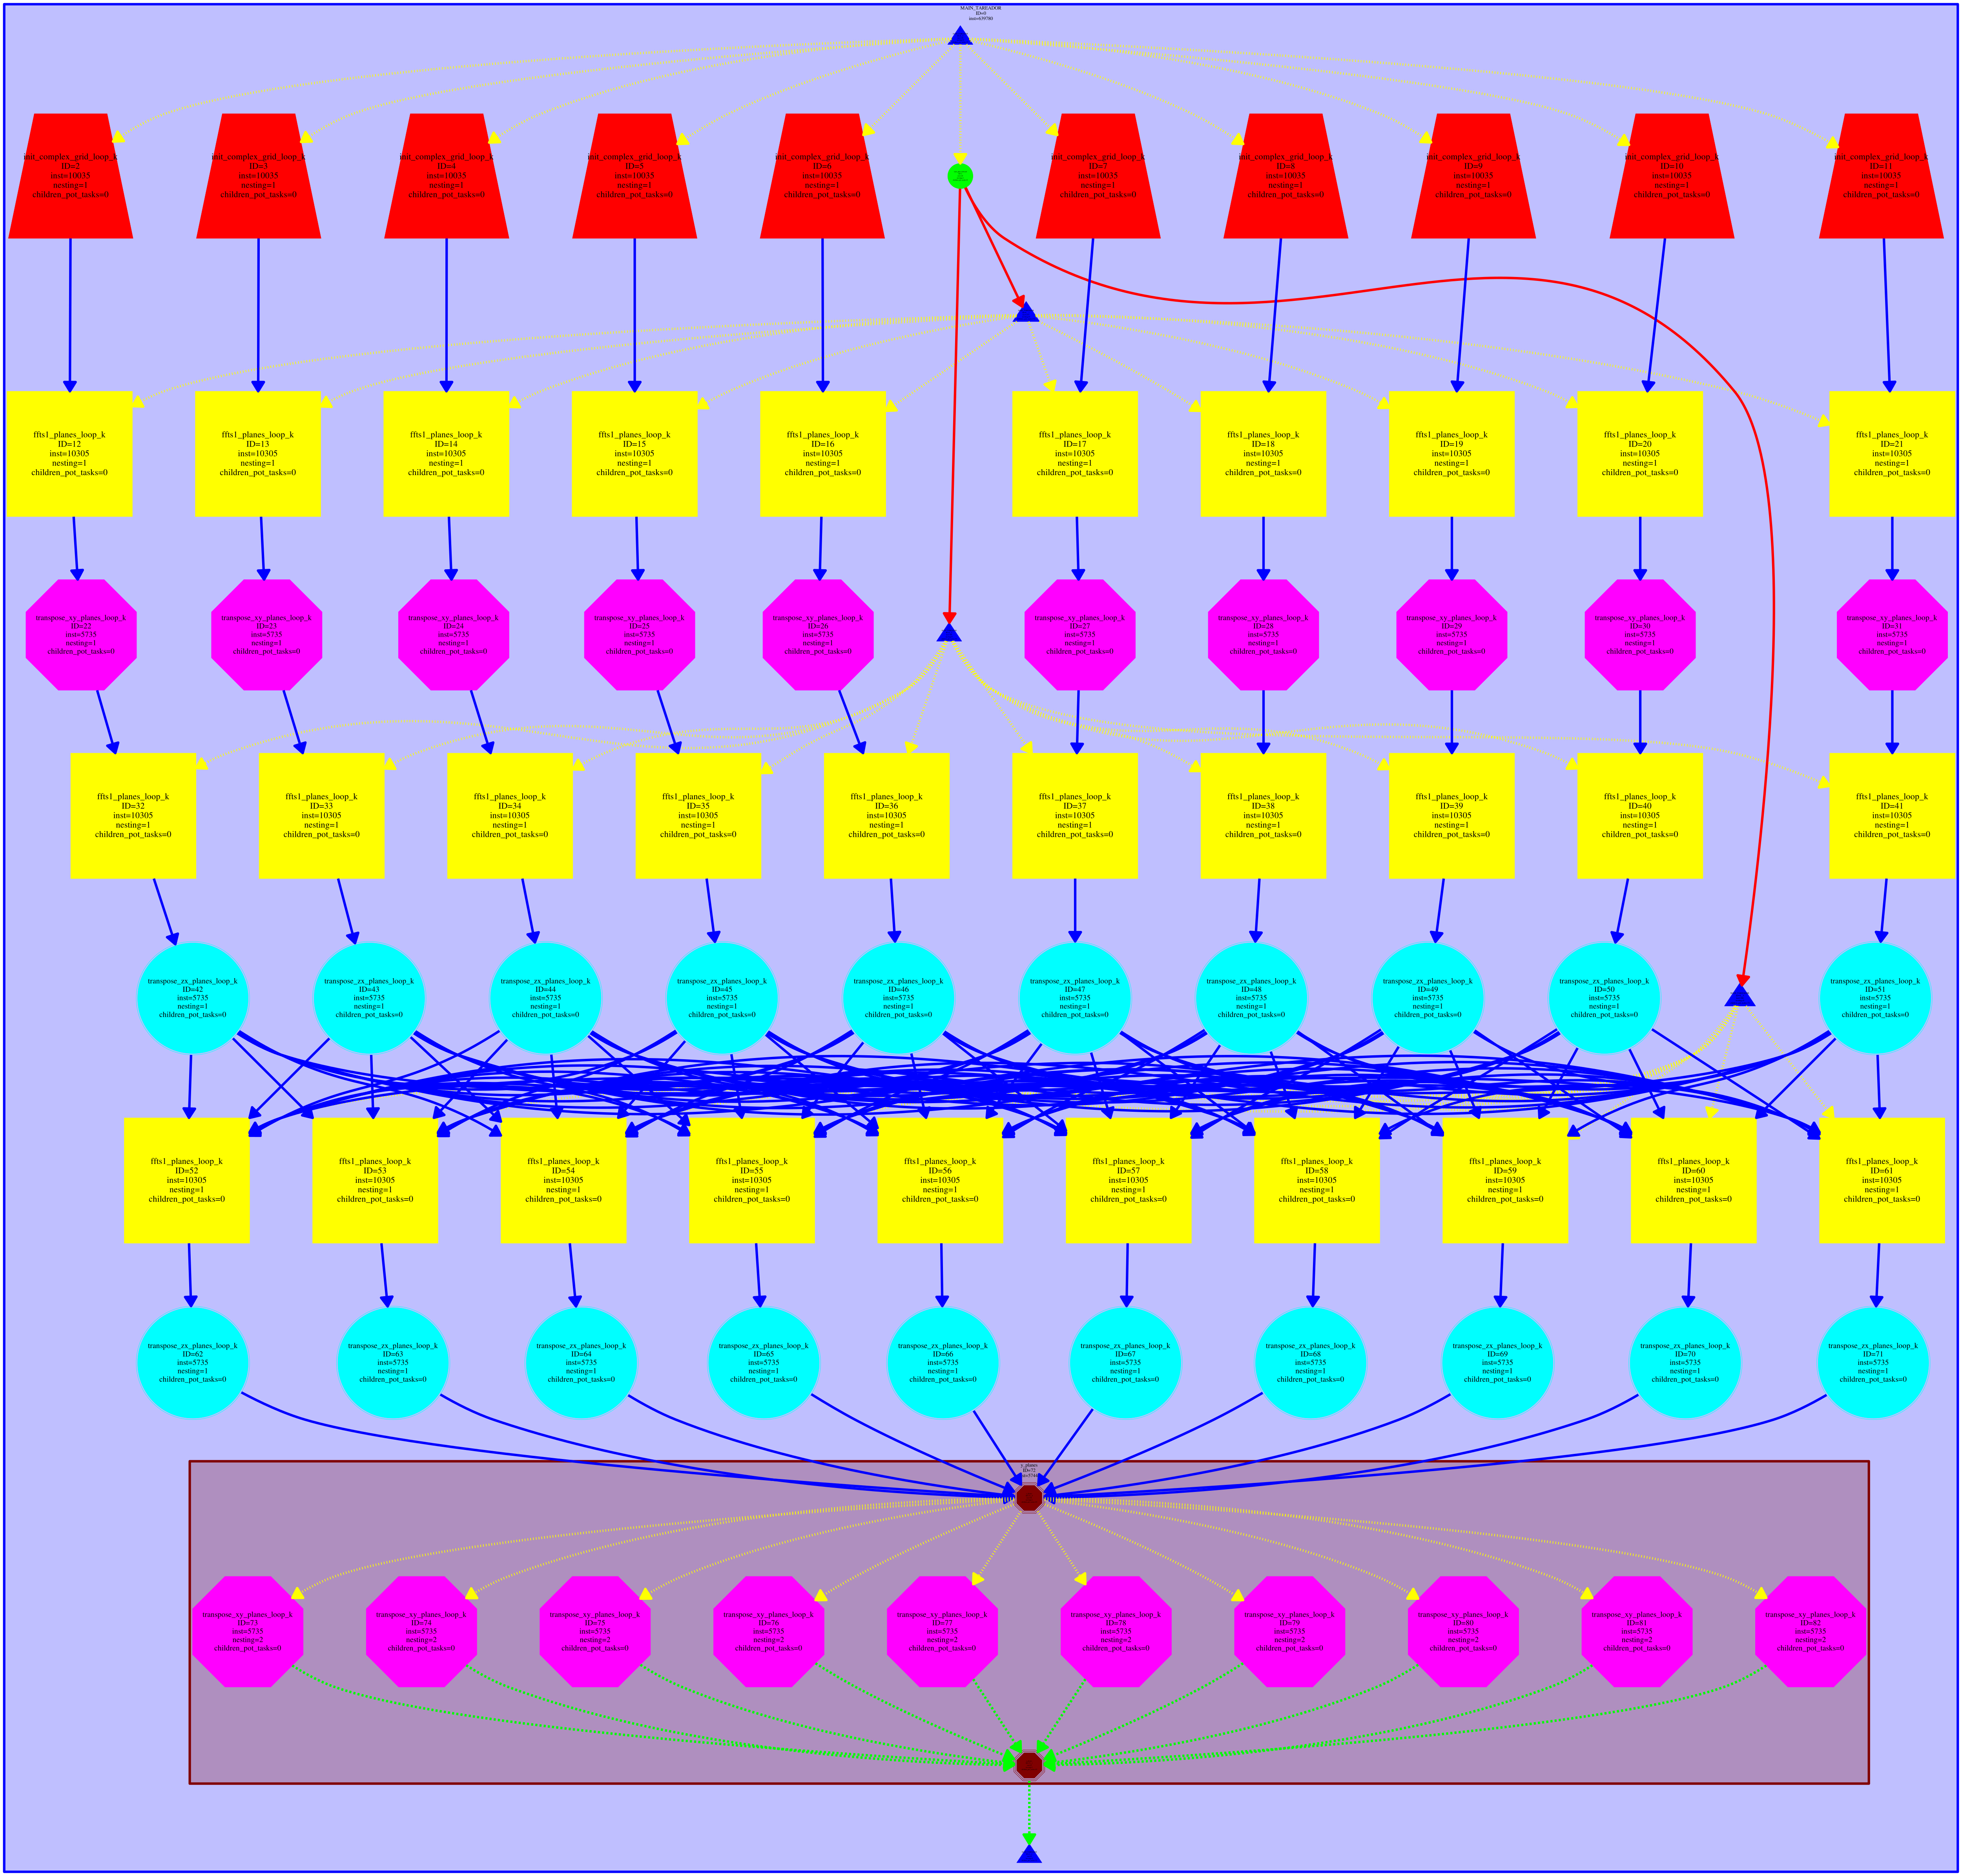
\includegraphics[width=0.3\textwidth]{data/3dfft_/plots/dependency_graph_v4.pdf.png}
    \caption{Dependency graph v4}%
    \label{fig:depen_v4}
\end{figure}
\begin{figure}[H]%
    \centering
    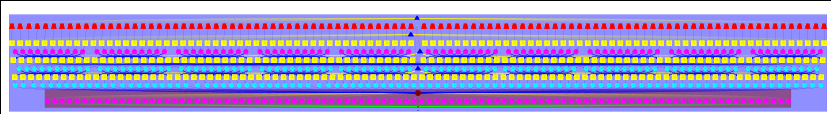
\includegraphics[width=\textwidth]{data/3dfft_/plots/cap.png}
    \caption{Dependency graph v5}%
    \label{fig:depen_v5}
\end{figure}

Figure~\ref{fig:diff} shows a portion of the differences between \emph{v4} and \emph{v5}. As we can see
the tasks of \emph{v5} are in a more inner part of the nested for loops (although not the deepest, there is 1 extra level we cold have tried), this means that \emph{v5} can have \emph{N} times more tasks than \emph{v4} for those methods, allowing for much higher parallelization as we have seen in figures~\ref{fig:exec_v4}-\ref{fig:exec_v5_log}.

\begin{figure}[H]%
    \centering
    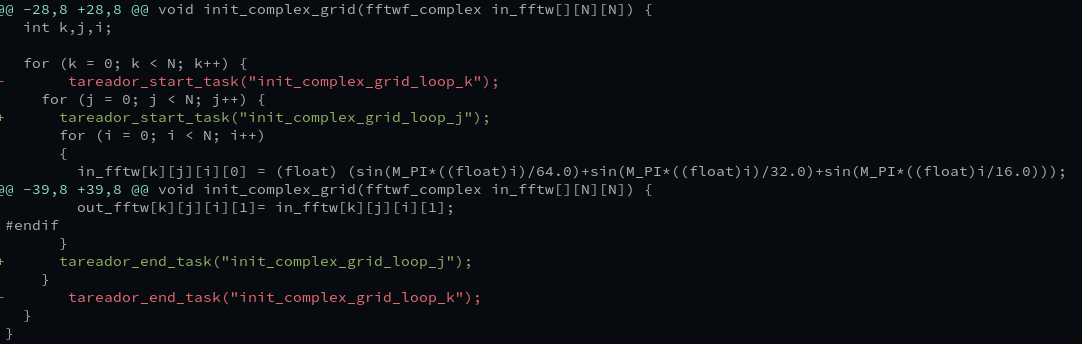
\includegraphics[width=\textwidth]{./data/3dfft_/plots/diff.png}
    \caption{Differences between v4 and v5}%
    \label{fig:diff}
\end{figure}

\begin{figure}[H]%
    \label{fig:plot_v4_01}
    \centering
    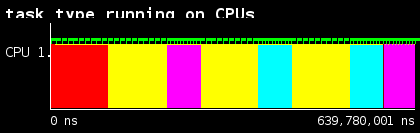
\includegraphics[width=0.49\textwidth]{./data/3dfft_/plots/v4_01.png}
    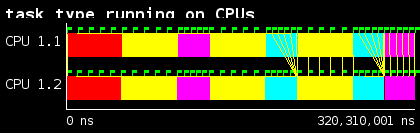
\includegraphics[width=0.49\textwidth]{./data/3dfft_/plots/v4_02.png}
    \caption{Execution time of v4 with 1 and 2 processors}%
\end{figure}

\begin{figure}[H]%
    \label{fig:plot_v4_04}
    \centering
    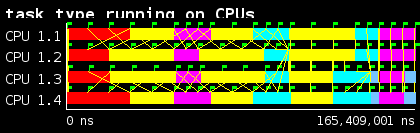
\includegraphics[width=0.49\textwidth]{./data/3dfft_/plots/v4_04.png}
    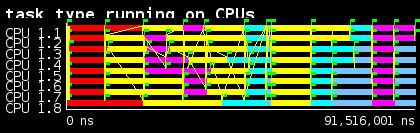
\includegraphics[width=0.49\textwidth]{./data/3dfft_/plots/v4_08.png}
    \caption{Execution time of v4 with 4 and 8 processors}%
\end{figure}

\begin{figure}[H]%
    \label{fig:plot_v4_16}
    \centering
    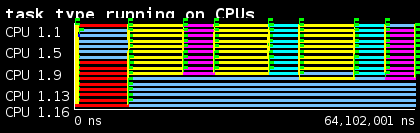
\includegraphics[width=0.49\textwidth]{./data/3dfft_/plots/v4_16.png}
    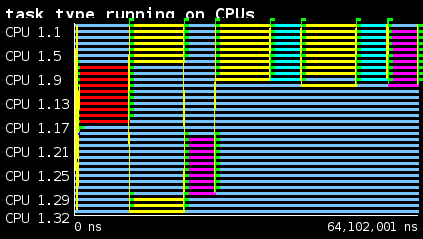
\includegraphics[width=0.49\textwidth]{./data/3dfft_/plots/v4_32.png}
    \caption{Execution time of v4 with 16 and 32 processors}%
\end{figure}

\begin{figure}[H]%
    \centering
    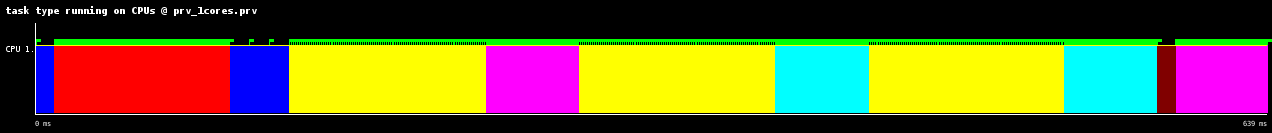
\includegraphics[width=0.49\textwidth]{./data/3dfft_/plots/v5_01.png}
    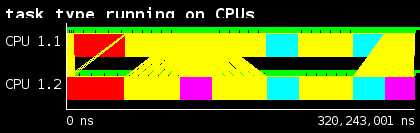
\includegraphics[width=0.49\textwidth]{./data/3dfft_/plots/v5_02.png}
    \caption{Execution time of v5 with 1 and 2 processors}%
    \label{fig:plot_v5_01}
\end{figure}

\begin{figure}[H]%
    \label{fig:plot_v5_04}
    \centering
    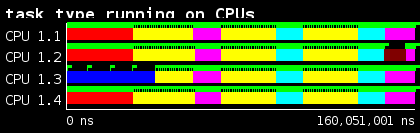
\includegraphics[width=0.49\textwidth]{./data/3dfft_/plots/v5_04.png}
    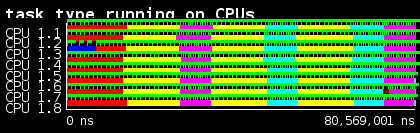
\includegraphics[width=0.49\textwidth]{./data/3dfft_/plots/v5_08.png}
    \caption{Execution time of v5 with 4 and 8 processors}%
\end{figure}

\begin{figure}[H]%
    \label{fig:plot_v5_16}
    \centering
    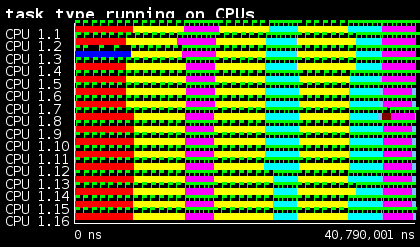
\includegraphics[width=0.49\textwidth]{./data/3dfft_/plots/v5_16.png}
    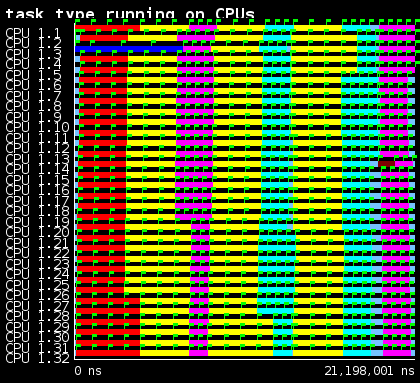
\includegraphics[width=0.49\textwidth]{./data/3dfft_/plots/v5_32.png}
    \caption{Execution time of v5 with 16 and 32 processors}%
\end{figure}


\section{Understanding the parallel execution of \emph{3DFFT}}%
\label{sec:understanding_the_parallel_execution_of_3dfft}

%In this final section of your report you should comment about how did you
%observed with Paraver the parallel performance evolution for the OpenMP
%parallel versions of 3DFFT. Support your explanations with the results reported
%in the following table which you obtained during the laboratory session. It is
%very important that you include the relevant Paraver captures (timelines and
%profiles of the % of time spent in the differentOpenMPstates) to support your
%explanations too.
% aunque tampoco se que hacer <--- BUSCA TODO:
\begin{table}[H]%
    \label{tab:under_parallelism}
    \centering
    %\caption{caption}
    \begin{tabular}{l
        S[table-format=1.3,round-mode=places,round-precision=3]
        S[table-format=2.3,round-mode=places,round-precision=3]
        @{\hskip 2em}
        S[table-format=10.0,round-mode=places,round-precision=3]
        S[table-format=10.0,round-mode=places,round-precision=3]
        S[table-format=1.3,round-mode=places,round-precision=3]
        }
    \toprule
    \thead{Version} & {$\phi$} & {$S_\infty$} & {$T_1$ (ns)} & {$T_8$ (ns)} & {$S_8$} \\
    \midrule
    initial version in \texttt{3dfft\_omp.c}                & 0.618754621 & 2.623294858 & 2519853052 & 1710690423 & 1.473003542 \\
    new version with improved $\phi$                        & 0.890828288 & 9.159881997 & 2365124299 & 955055104 & 2.47431528 \\
    final version\footnotemark     & 0.903348138 & 10.346412184 & 2401885497 & 626806635 & 3.831940128 \\
    \bottomrule
    \end{tabular}
\end{table}
\footnotetext{with reduced parallelization overheads}

\begin{figure}[H]%
    \centering
    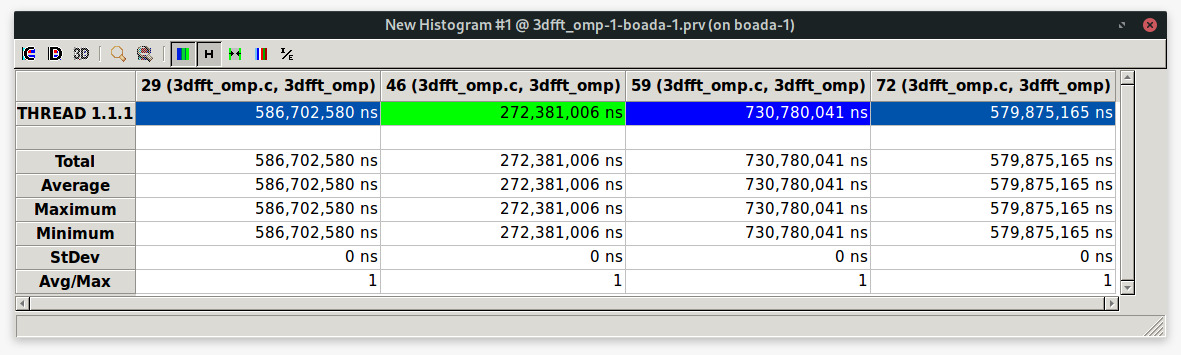
\includegraphics[width=\textwidth]{./data/omp1.jpeg}
    \caption{2DAnalyzer window of the initial version with the parallel functions cfg}%
    \label{fig:omp1}
\end{figure}

\begin{figure}[H]%
    \centering
    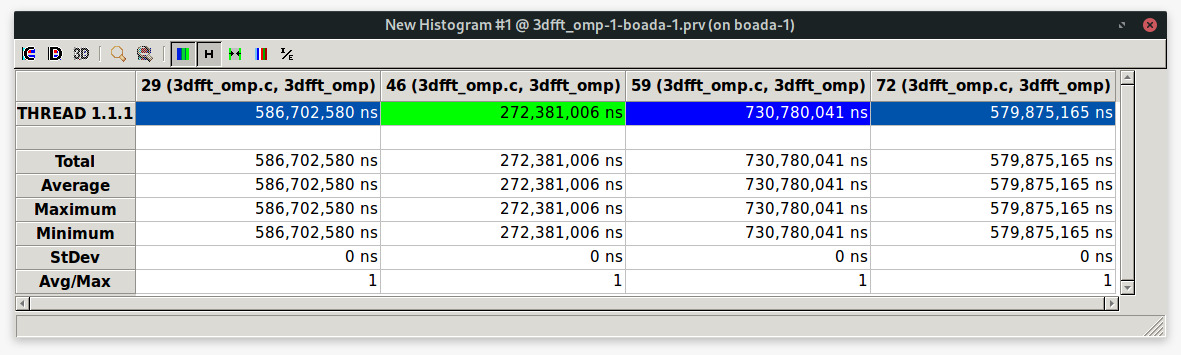
\includegraphics[width=\textwidth]{./data/omp2.jpeg}
    \caption{2DAnalyzer window of the improved version with the parallel functions cfg}%
    \label{fig:omp2}
\end{figure}

\begin{figure}[H]%
    \centering
    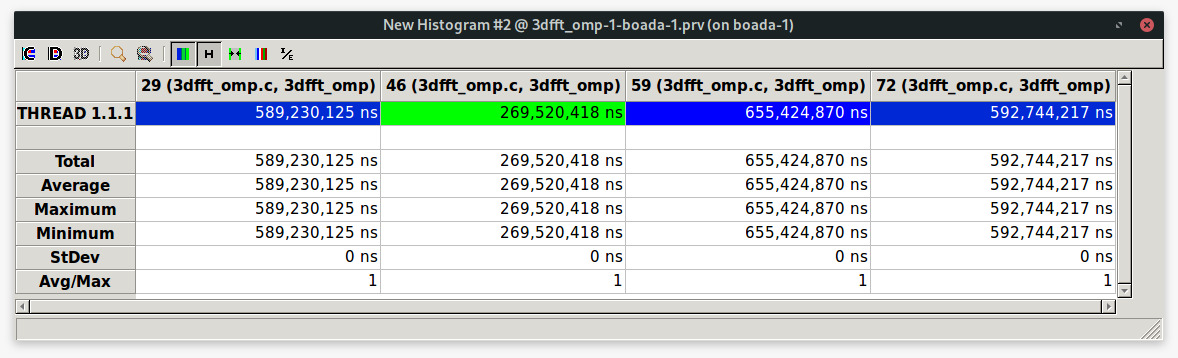
\includegraphics[width=\textwidth]{./data/omp3.jpeg}
    \caption{2DAnalyzer window of the final version with the parallel functions cfg}%
    \label{fig:omp3}
\end{figure}

%TODO: comment about how did you observed with Paraver the parallel 
%      performance evolution for the OpenMP parallel versions of 3DFFT.

%Finally you should comment about the (strong) scalability plots (execution time
%and speed–up) that are obtained when varying the number of threads for the
%three parallel versions that you have analysed.

\begin{figure}[H]%
    \centering
    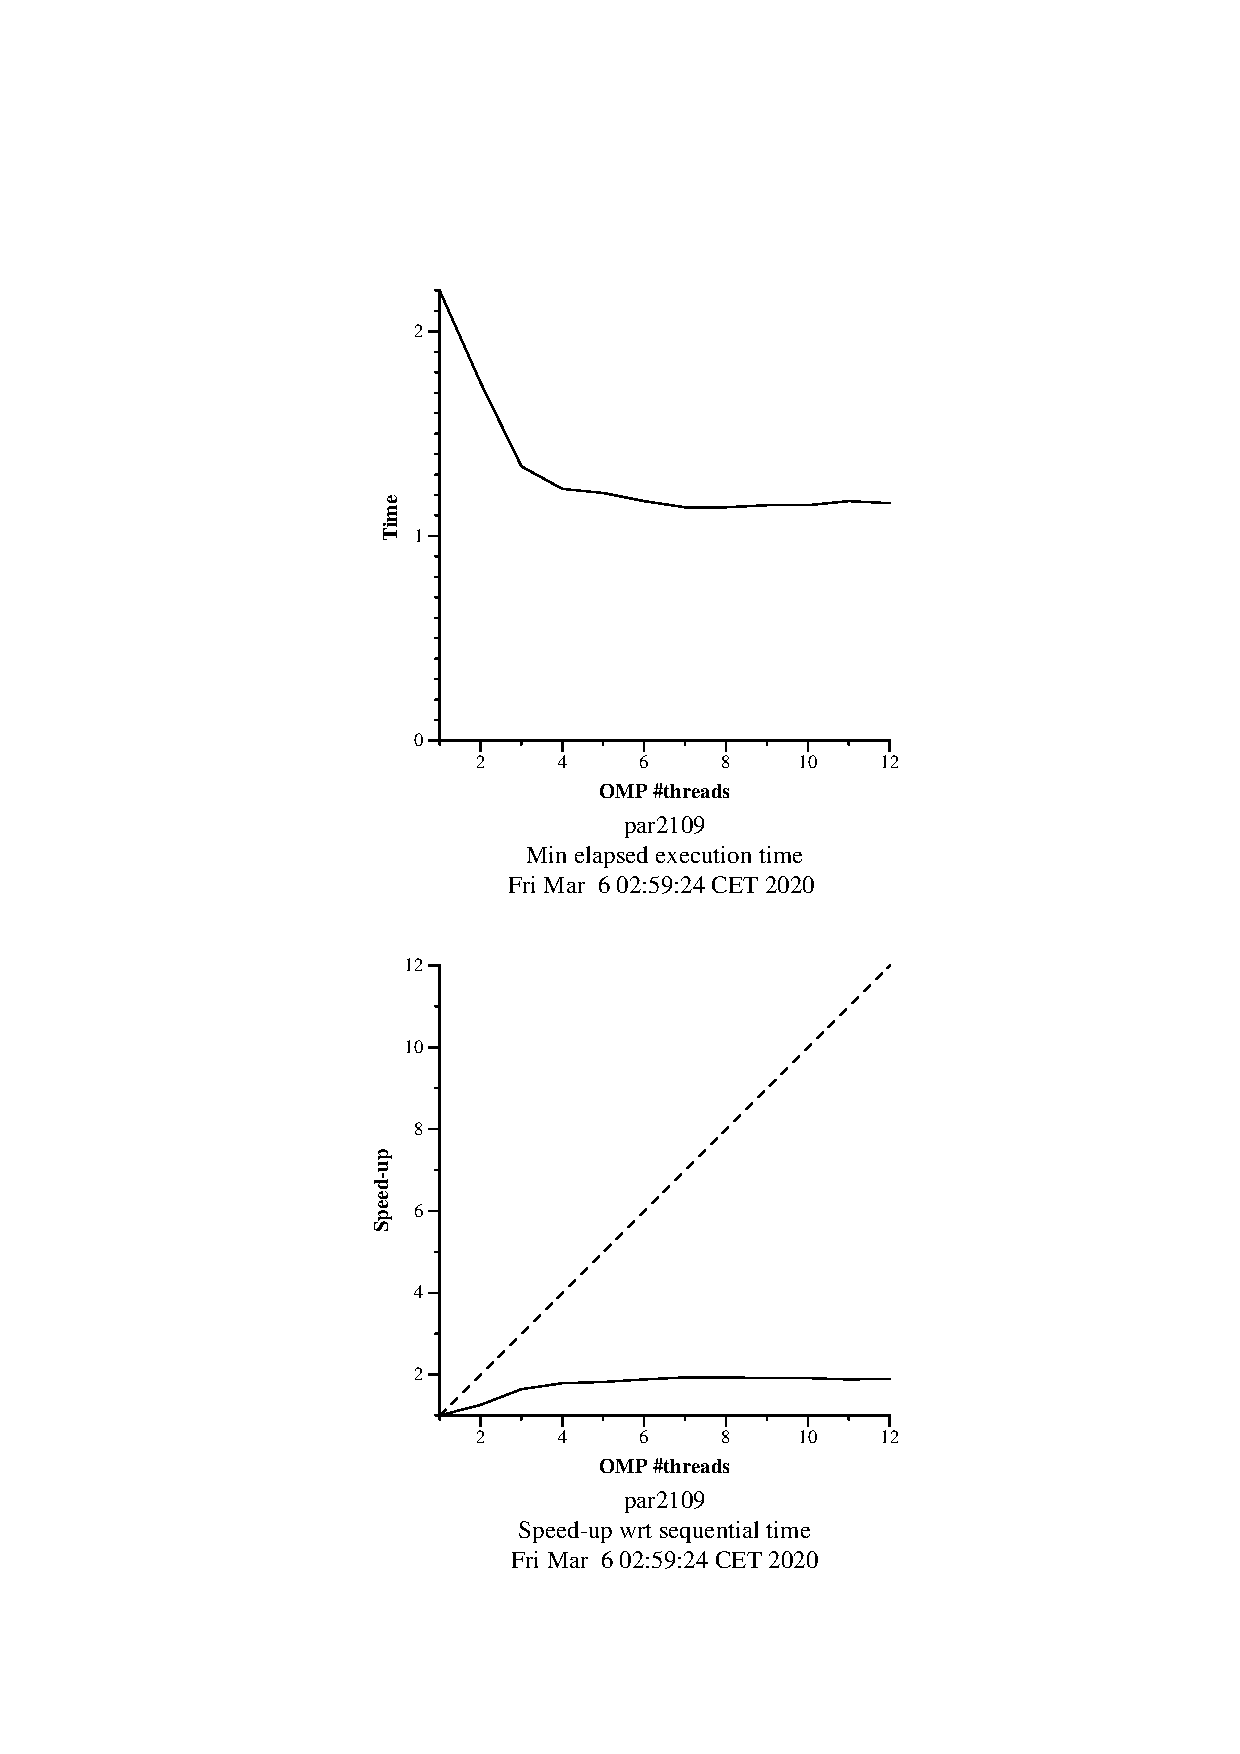
\includegraphics[width=\textwidth]{./data/3dfft_/3dfft_omp-strong-1.pdf}
    \caption{Strong scalability of the initial version}%
    \label{fig:omp1-plot}
\end{figure}

\begin{figure}[H]%
    \centering
    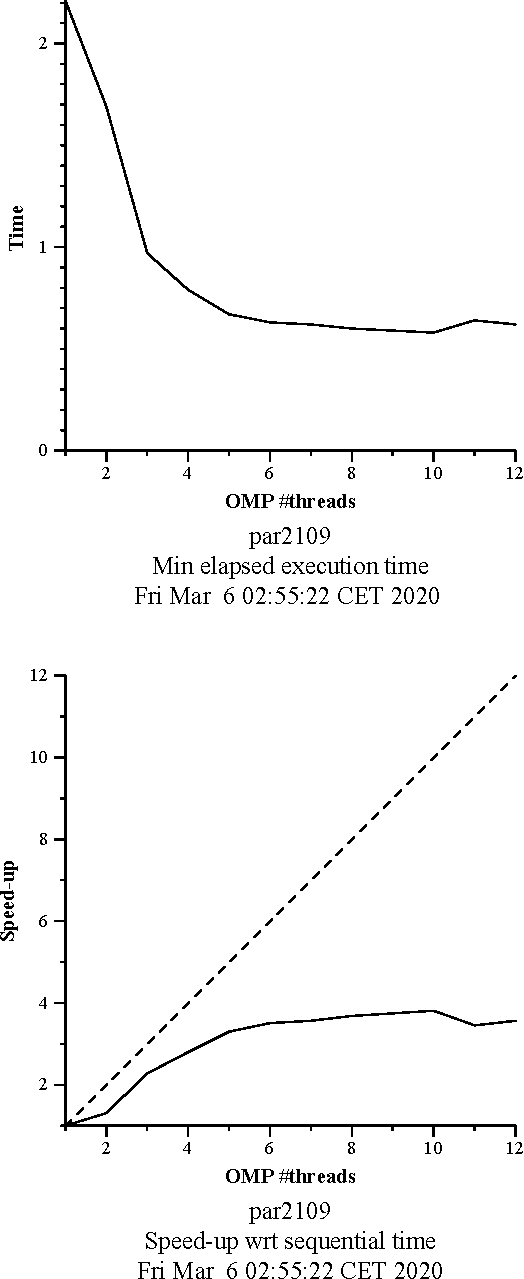
\includegraphics[width=\textwidth]{./data/3dfft_/3dfft_omp-strong-2.pdf}
    \caption{Strong scalability of the improved version}%
    \label{fig:omp2-plot}
\end{figure}

\begin{figure}[H]%
    \centering
    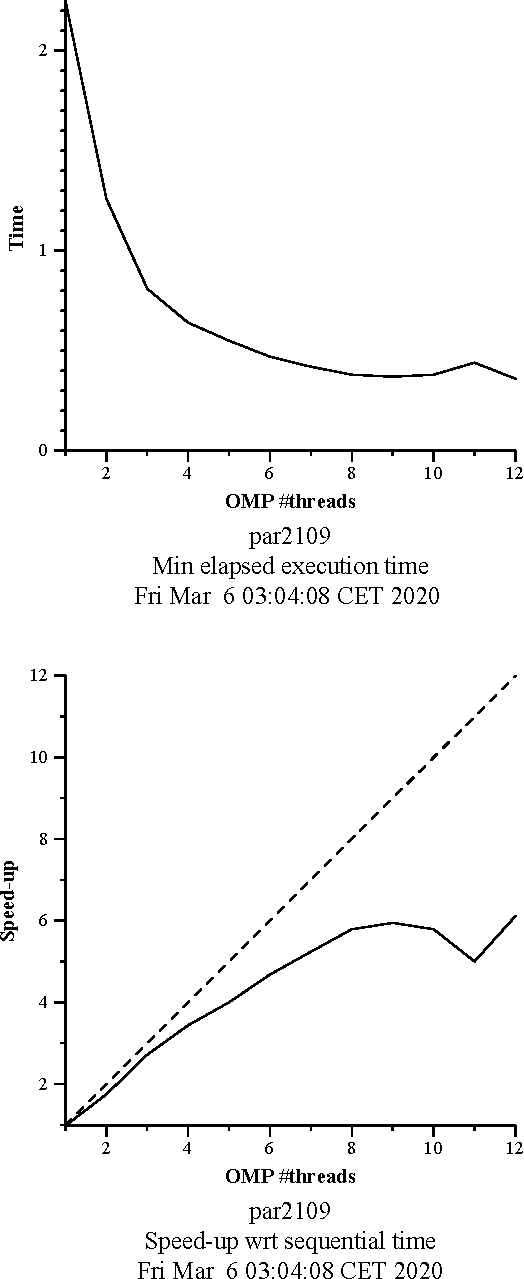
\includegraphics[width=\textwidth]{./data/3dfft_/3dfft_omp-strong-3.pdf}
    \caption{Strong scalability of the final version}%
    \label{fig:omp3-plot}
\end{figure}

%TODO: comentar los plots

\end{document}
